\documentclass{article}
\usepackage[utf8]{inputenc}

\usepackage[colorlinks]{hyperref}
\usepackage{multicol}
\usepackage{geometry}
 \geometry{
 letterpaper,
 total={100mm,230mm},
 left=60mm,
 top=20mm,
 }
% Used by the template
\usepackage{setspace}
\usepackage{changepage} % to adjust margins
\usepackage[breakable]{tcolorbox}
\usepackage{float} % for tables inside tcolorbox https://tex.stackexchange.com/a/274342
\usepackage{enumitem}
\usepackage{subfigure}


\begin{document}

% Each section is supposed to be brief, in the form of a bullet list.
% This environment formats the lists in each model card section in a compact format to help
% the card fit into the recommended "one to two pages".
\newenvironment{mcsection}[1]
    {%
        \textbf{#1}

        % Reduce margins to use the space more effectively and help fit in the recommended "one to two pages"
        % Use the bullet list format as shown in the model card paper to increase readability
        \begin{itemize}[leftmargin=*,topsep=0pt,itemsep=-1ex,partopsep=1ex,parsep=1ex,after=\vspace{\medskipamount}]
    }
    {%
        \end{itemize}
    }

% Optional: reduce margins single line to fit in "one to two pages", as recommendedhttps://www.overleaf.com/project/6048b469ca0a6b076ff8cce9
\begin{adjustwidth}{-90pt}{-80pt}
\begin{singlespace}

\tcbset{colback=white!10!white}
\begin{tcolorbox}[breakable, sharp corners, boxrule=0.7pt]
\begin{center}
    \large\textbf{Model Card - Stock Price Direction Prediction}
\end{center}
% Change to a smaller, but still legible font size to help fit in the recommended "one to two pages"
\small{
\begin{multicols}{2}
\begin{mcsection}{Model Details}
    \item Developed by students at the Université de Montréal, 2021, v1.
    \item Logistic Regression.
    \item Trained to predict the stock price based on the historical data for binary price direction classification.
\end{mcsection}

\begin{mcsection}{Intended Use}
    \item Intended to be used for trading application which allows to trade, view latest quotes, track your portfolio and also predicts the performance of the stocks.
    \item Model performance is subjected to Market conditions, so users should be aware of associated risks.
    \item Intended for customers who are active traders.
    \item Not intended to determine the stock market performance. Stocks direction were predicted based on historical data.
\end{mcsection}

\begin{mcsection}{Factors}
    \item Evaluation is based on known attributes of stock namely Price, Return, Lag\textunderscore1, Lag\textunderscore2, Lag\textunderscore3, Lag\textunderscore4, Momentum and Moving average.
\end{mcsection}

\begin{mcsection}{Metrics}
    \item Evaluation metrics include Historical Daily price of stocks, Confusion Matrix to measure model performance based on Actual and Predicted data. True Positive and False Postive metries are generated and further used to show AUC - ROC curve to determine asses model performance. The AUC-ROC curve are generated using Train data, Test data and Population Data and bench-marked against Random Classifier.
\end{mcsection}

\begin{mcsection}{Training Data}
    \item Alphabet stock(GOOG) pricing data starting from 1st January 2017 to 1st January 2018, training data split: 50\% shuffled randomly.
\end{mcsection}

\begin{mcsection}{Evaluation Data}
    \item Alphabet stock(GOOG) pricing data starting from 1st January 2017 to 1st January 2018, test data split: 50\% shuffled randomly.
\end{mcsection}

\begin{mcsection}{Ethical Considerations}
    \item Stock market data based on the actual data from the internet. No new information is inferred or annotated.
\end{mcsection}

\begin{mcsection}{Caveats and Recommendations}
    \item Model input data only includes stock market close prices and derived features. The macro-economic variables such as interest rates, market volatility and other factors such as latest news, market sentiments are not included.
\end{mcsection}

\end{multicols}

\textbf{Quantitative Analyses}
\begin{figure}[H]
\centering
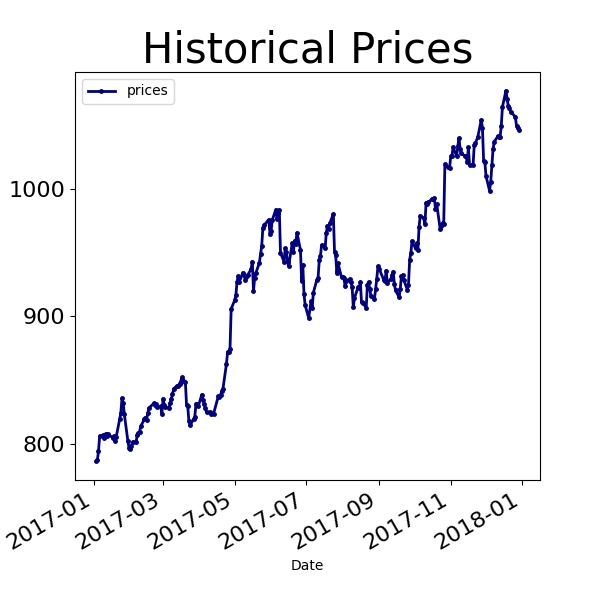
\includegraphics[width=.3\linewidth]{prices.png} \space \space
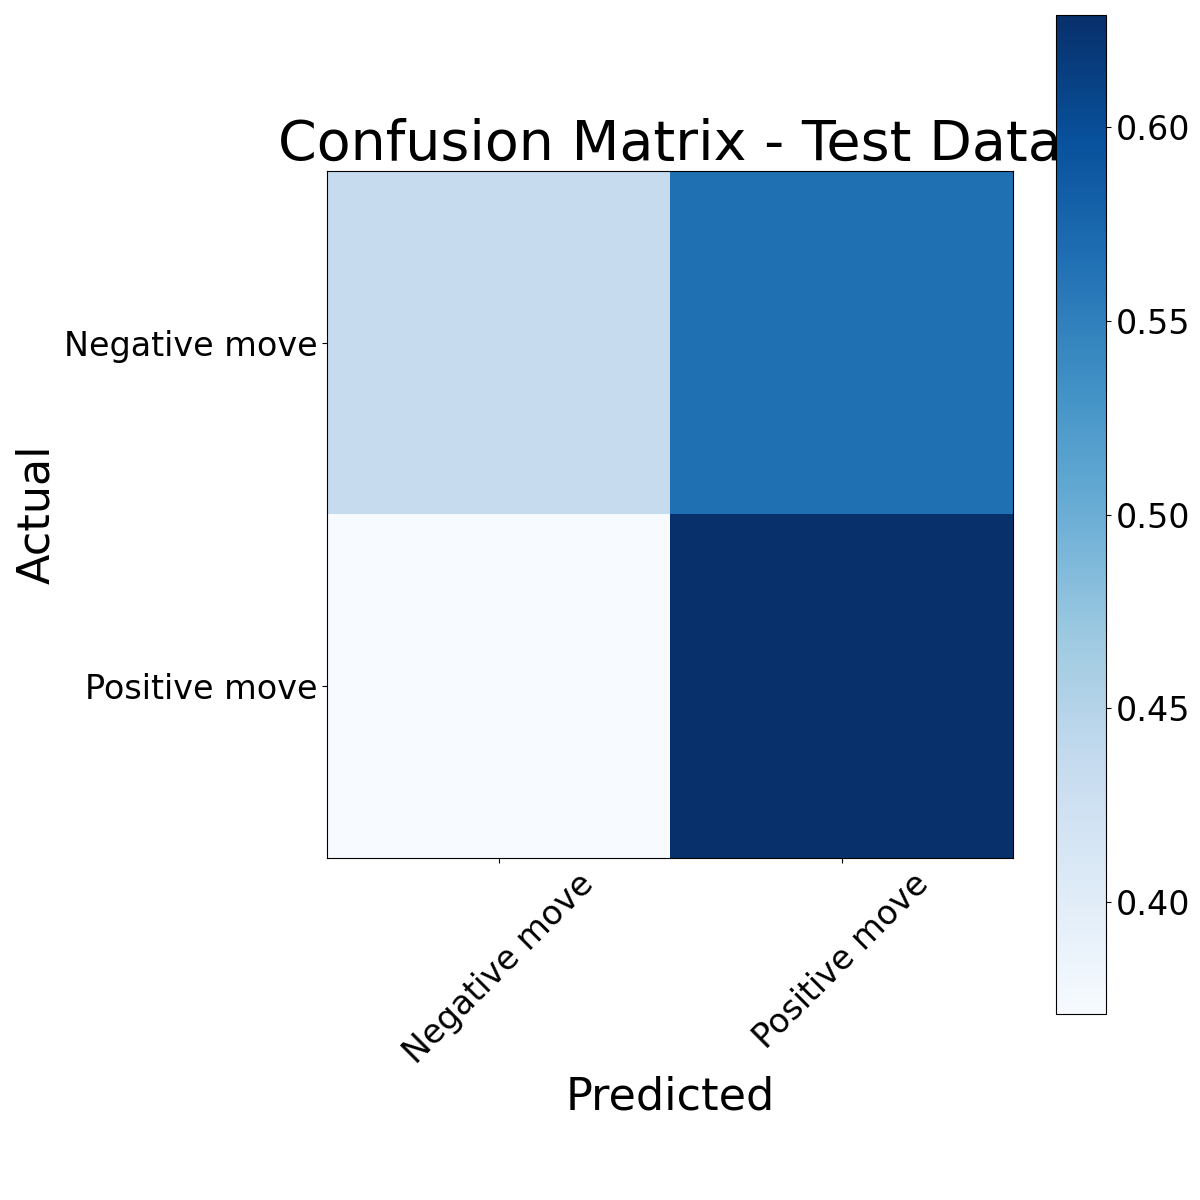
\includegraphics[width=.3\linewidth]{confmatrix.png} \space \space
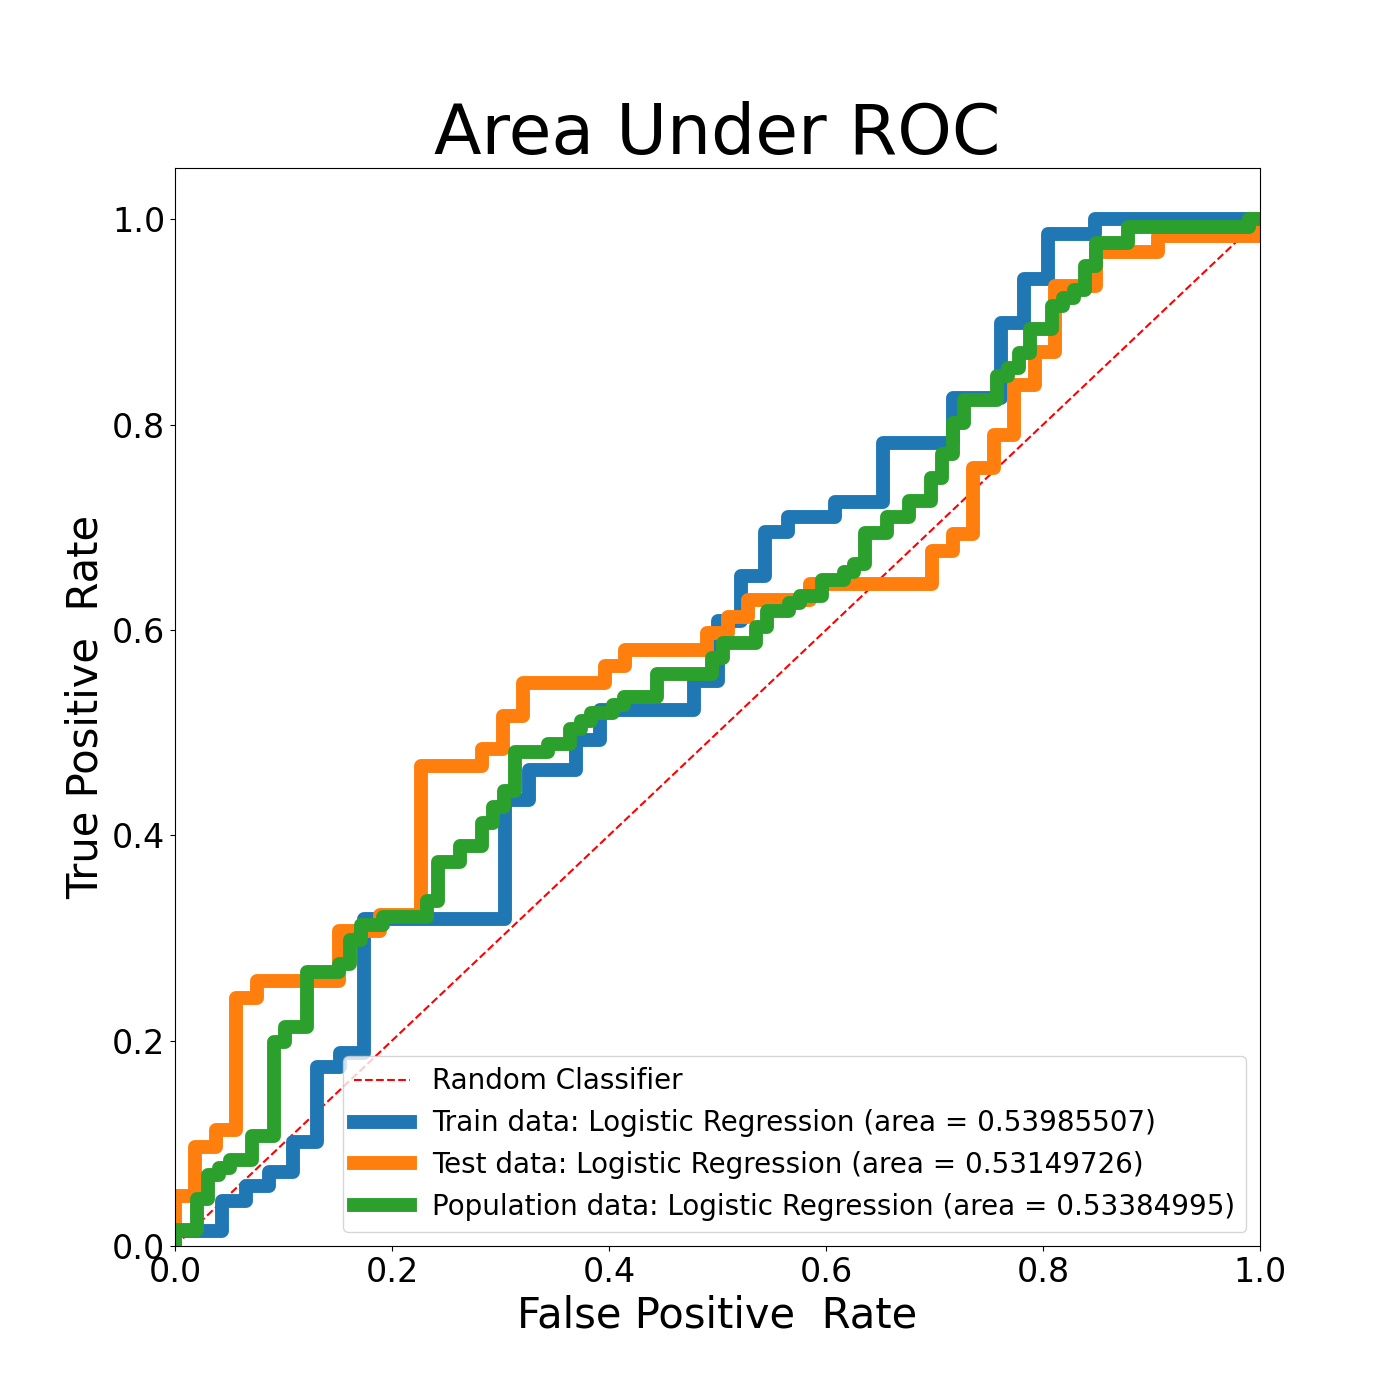
\includegraphics[width=.3\linewidth]{roc.png}
\end{figure}

} % end font size change

\end{tcolorbox}

\end{singlespace}

\end{adjustwidth}

\end{document}
